\section{Model fit coefficients}

\subsection{Fitting}

\begin{figure}
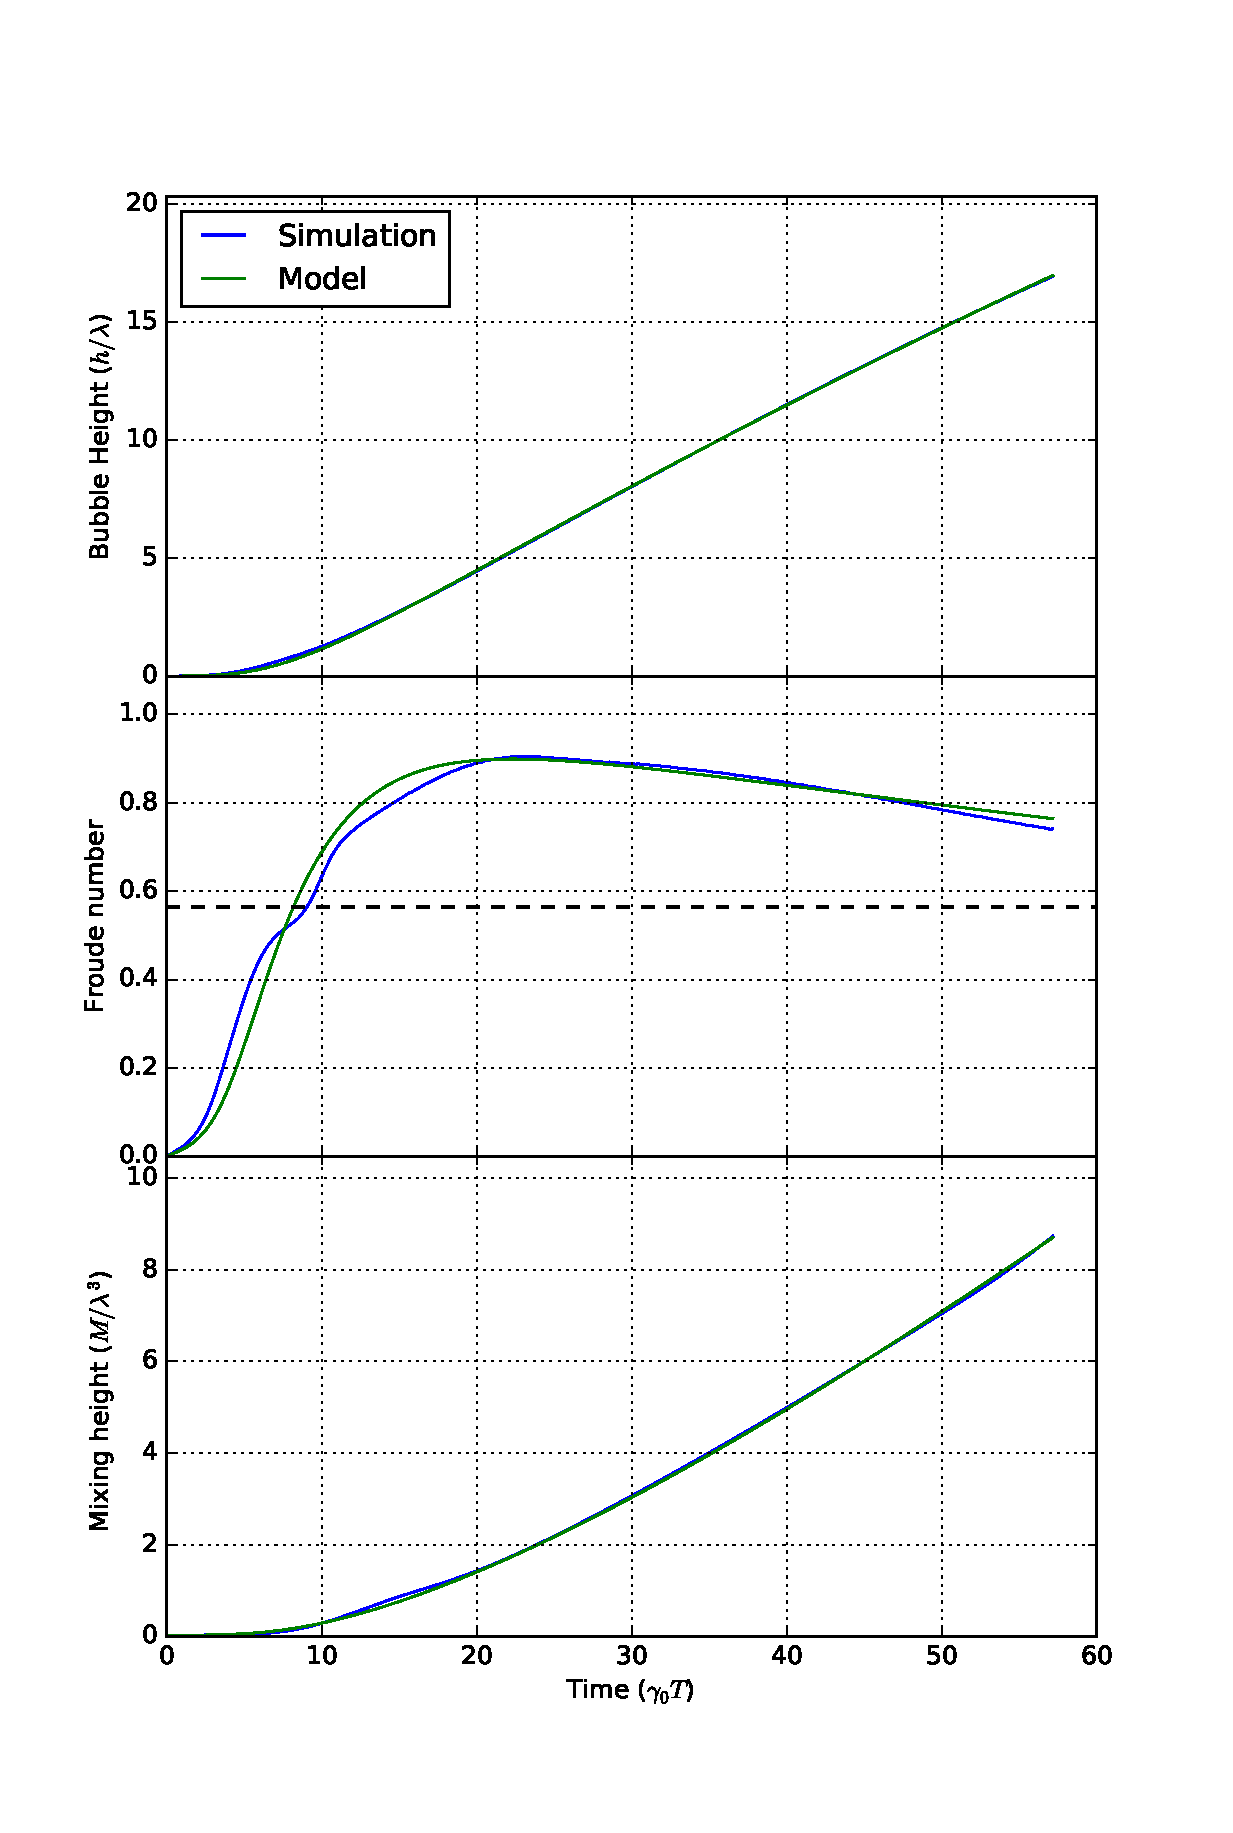
\includegraphics[width=\columnwidth]{figs/H-8-1}
\caption{ \flabel{example_fit}
  Example fit of the bubble height, top, and mixed volume, bottom, at $\text{Ra} = $ and $\text{Sc} = 8$.
  The Froude number, which is a non-dimensional velocity, is not directly fit but shows agreement between the model and simulation.
}
\end{figure}

The mixing model defines the quantity of mixed fluid, $m(t)$, as an analytic function:
\begin{equation}
\left\{H(t), \delta(0), \lambda, D, C_5\right\} \rightarrow m(t),
\end{equation}
where $H(t)$ is the buble height, 
$\delta(0)$ is the initial interface thickness,
$\lambda$ is the wavelength,
$D$ is the diffusivity, and 
$C_5$ is a mixing coefficient.
The values of $H(t)$, $\delta(0)$, $\lambda$, and $D$ are taken from the numerical experiments, allowing for the definition of an mixing error:
\begin{equation}
E_m = \left|\left|m\left[C_5\right] - M(t) \right| \right|_2,
\end{equation}
where $M(t)$ is the reference value from the numerical experiments.
To compute $C_5$, the error is minimized under the constraint $C_5 > 0$.
The fitting problem is non-linear but 1D dimensional, so it can be solved with a sequential least squares minimizer, which finds local minima, wrapped with a basin hopping scheme, which samples across the local minima.

The dynamics model defines the bubble height, $h(t)$, as the solution to an ordinary differential equation.
The dynamics model is integrated using the variable-coefficient ordinary differential equation (VODE) solver for stiff systems, creating a map from the dynamics coefficients to the height:
\begin{equation}
\left\{h(0), \delta(0), \lambda, \nu, D, C\right\} \rightarrow h(t),
\end{equation}
where $h(0)$ is the initial bubble height,
$\delta(0)$ is the initial interface thickness,
$\lambda$ is the wavelength,
$\nu$ is the kinematic viscosity,
$D$ is the diffusivity, and
$C$ are the model cofficients.
$\delta(0)$, $\lambda$, $\nu$, and $D$ are taken from the simulation while $C_5$ is taken from independently fitting the mixing model, allowing for the definition of a dynamics error:
\begin{equation}
E_d = \left| \left| h\left[C_1, C_2, C_3, C_7\right] - H(t)\right| \right|_2,
\end{equation}
where $H(t)$ is the reference value from the numerical experiments.
The non-linear global minimization problem is solved with the covariance matrix adaptation evolution strategy (CMA-ES).
CMA-ES iteratively refines a sample distribution that evolves towards the global optimum.
Computing the model error is very inexpensive compared to the simulations, so we choose a broad initial distribution with a large population size.
The stocastic solution is polished with a sequential least-squares local minimization.

However, the high Rayleigh trajectories are incomplete, in that the data ends when the bubble gets close to the top wall, leading to underconstrained systems.
Therefore, we regularize the fit by adding a term to the model error:
\begin{equation}
R = \beta \left| \left| \frac{C - \bar{C}}{\bar{C}} \right| \right|_2,
\end{equation}
where $\beta$ is the regularization parameter,
$C$ is the vector of model coefficients, and
$\bar{C}$ are the coefficient estimates.
Although the buoyancy-drag model is non-linear, this L2 regularization can be thought of as a Tikhonov regularization or Ridge Regression.
The regularization parameter is chosen to be an order smaller than the model error, $\beta = 0.1 E_d$.
The if the regularized dynamic error ends up lower than the unregularized error, the unregularized problem must not have converged to the local minima.
In those cases, the unregularized fit is repeated with the regularized coefficient values as a starting seed.
Then the regularized fit is repeated with the updated definition.
In this way, the two types of fits are iterated until consistency is reached.

The fitting process defines a mapping from the Grashof and Schmidt numbers to the model coefficients and model errors:
\begin{equation}
\left(\text{Gr}, \text{Sc}\right) \rightarrow \left(C_1, C_2, C_3, C_5, C_7, E_m, E_d\right) 
\end{equation}
The rest of this section explores the relationships in this mapping.

\subsection{Scope of the models}

The proposed models aim to describe the mixing and dynamics in rising Rayleigh-Taylor bubbles and falling Rayleigh-Taylor spikes.
The symmetry of the governing equations equates the spike behavior to that of the bubbles, so we will omit spikes from the following discussions.
In highly viscous and diffusive cases, the bubbles may not reach late time highly non-linear dynamics.
For this analysis, a bubble is considered to be covered by the model only if its height exceeds its wavelength before it stops rising.
Experiments which do not meet that condition are discarded.

The bubble grows until mixing dillutes its buoyancy sufficiently for it to stop rising.
After this point, it slowly receeds due to diffusing across the bubble tip.
The model does not account for this diffusive effect, which moves move the center of the interface rather than just broaded it, so bubble trajectories are clipped beyond the point at which the bubble velocity is zero.
The height at that point in the trajectory is maximal and called the \textit{penetration depth}.

The penetration depth increases with Rayleigh number.
For high Rayleigh number cases, the bubble continues to grow until it beings to interact with the top boundary, given the finite computational domain.
Based on previous validation studies~\cite{Hutchinson2016}, we clip the trajectory when the bubble height reaches 75\% of the domain height.
Experiments in which this clipping occurs are incomplete.
Those cases should be re-simulated with a larger computational domain, at greater computational cost, to collect trajectories which reach their penetration depth.

However, there is still information in the incomplete experiments.
In the following sections, incomplete experiments will be marked as such, but the trend in the complete experiments is often seen to continue smoothly into incomplete ones.
Though not definitive, those suggest that the data present in the incomplete experiments is sufficient to constrain the corresponding characterization of the flow.
Conversely, in some cases the behavior in the incomplete experiments departs from that in the complete ones. 
In those cases, it is difficult to differentiate between Rayleigh-dependent behavior and the side-effects of underconstrained fitting.

\subsection{Accuracy of the models}

\begin{figure*}
\begin{subfigure}[b]{\columnwidth}
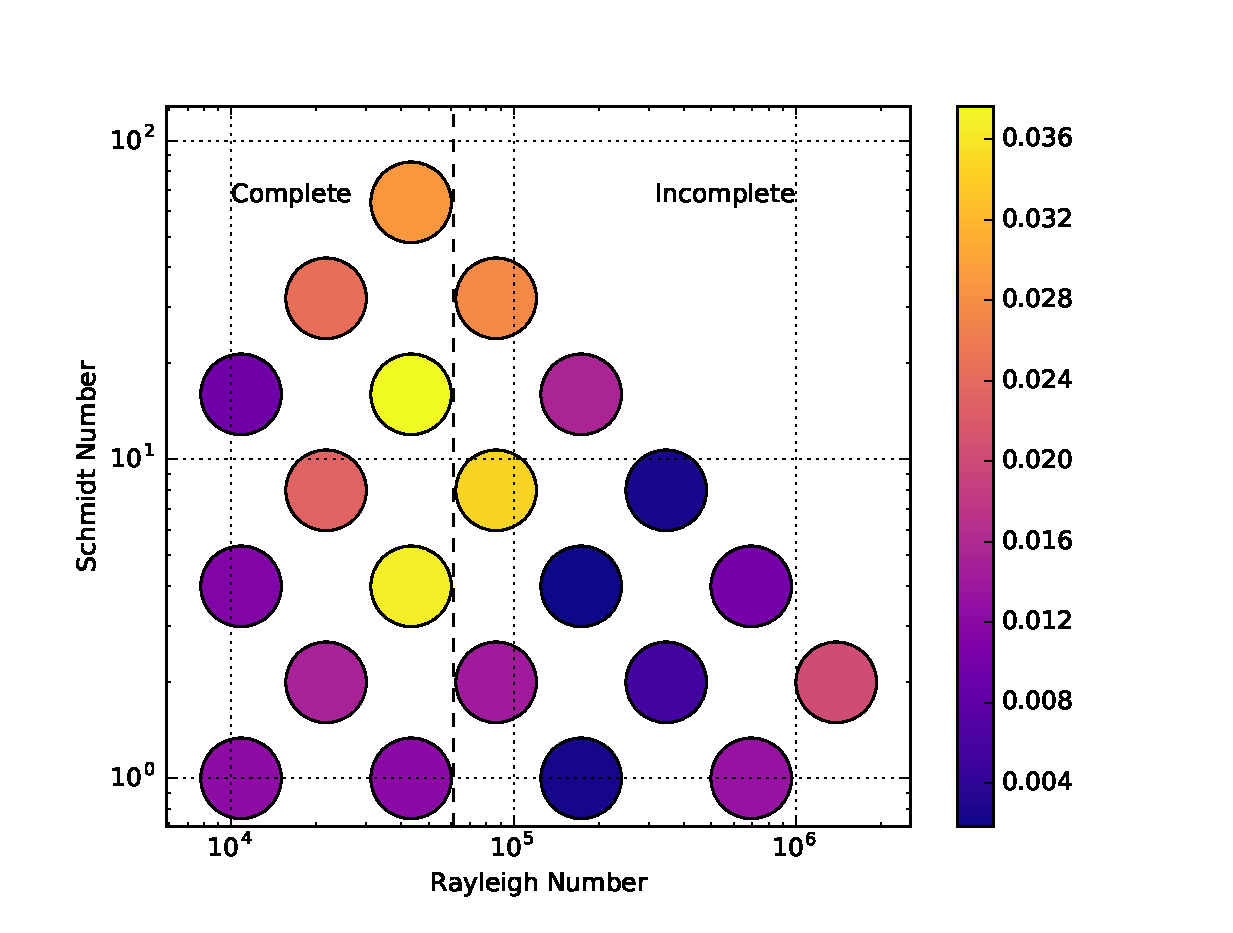
\includegraphics[width=\columnwidth]{figs/MixingError-vs-Rayleigh-Schmidt}
\caption{Relative mixing error, $E_m/\text{max}[M(t)]$}
\end{subfigure}
\begin{subfigure}[b]{\columnwidth}
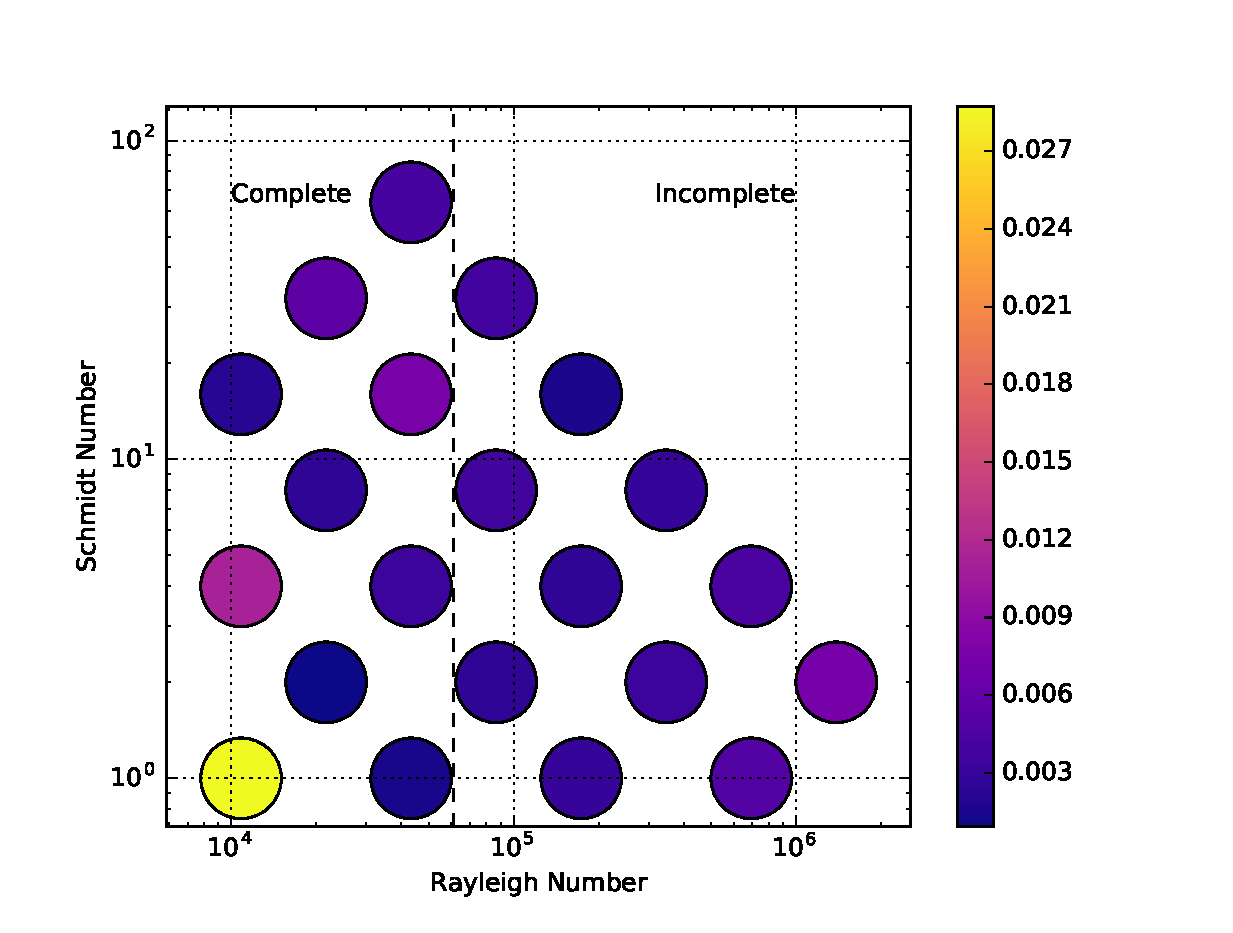
\includegraphics[width=\columnwidth]{figs/DynamicsError-vs-Rayleigh-Schmidt}
\caption{Relative dynamics error, $E_d/\text{max}[H(t)]$}
\end{subfigure}
\caption{ \flabel{errVsParam}
  Relative model errors vs Rayleigh and Schmidt numbers.
  Experiments on the left side of the dashed line completed when the bubble stopped rising.
  Experiments on the right side of the dashed line are incomplete, having approached the vertical boundaries of the simulated domain.
}
\end{figure*}

The accuracy is characterized by the mixing and dynamics model errors relative to the maximum mix volume and bubble height, respectively.
The relative model errors are plotted vs the Rayleigh and Schmidt numbers in \fref{errVsParam}.
In both models, the nominal error is less than 5\%, but the two errors have differing structures.

The relative mixing error is about 3\% for the complete experiments, with generally greater relative error at greater Rayleigh and Schmidt numbers.
Amoung the incomplete experiments, relative error decreases with Rayleigh number before increasing again.
This is likely due to the incompleteness; the greater error above $\text{Ra} = 10^6$ suggests that the overall trend is increasing.
Overall, the relationship between the accuracy of the mixing model the Rayleigh and Schimdt numbers is incomplete.

The relative dyanmics error is about 1\%, with the exception of the unit Schmidt $\text{Ra} \approx 10^4$ case.
The mixing error for the outlying case is typical, so the error cannot be attributed to the treatment of mixing.
This case will be considered more in the following sections.
Outlier aside, the relative error decreases with Schmidt number and Rayleigh number, both for complete and incomplete trajectories.
This indicates the dynamics model is most accurate, at least relative to the mixing height, when there is less mixing and drag.
Another factor is reacceleration, which adds some relatively constant error that is amortized more when the penetration depth is greater.


\begin{comment}
The model proposed in \sref{model} assumes the bubble is a coherent structure with a single velocity.
If the Grashof number is high, then the bubble can break up into multiple smaller bubbles as the bubble accelerates.
The break-up is easily identified visually.
Increasing the Grashof number, Schmidt number, or both should enhance the break-up, so we can identify a bifurcataion boundary for the break-up.

On the other hand, at low Grashof and Schmidt numbers, the growth of bubble height can be dominated by the growth of the interface widith, leading to predominantly diffusive dynamics.
This is particularly evident when the bubble height receeds, a process which is not accounted for in the buoyancy-drag model.
When the bubble velocity reverses, the trajectory is truncated for the purposes of fitting.
We can identify cases for which the bubble height receeds over the first time unit.
Similar to the break-up, decreasing the Grashof number, Schmidt number, or both should supress the bubble growth, so we can identify a bifurcation boundary here as well.
\end{comment}


\subsection{Fit coefficients}
The proposed model has 5 undetermined parameters.
In each case, we estimate the value a-priori by physical arguments.
Then, the estimates are used as the starting point for fitting, that is minimization of the model error over the scope of the model.

\subsubsection{Form drag coefficient, $C_1$}

\begin{figure}
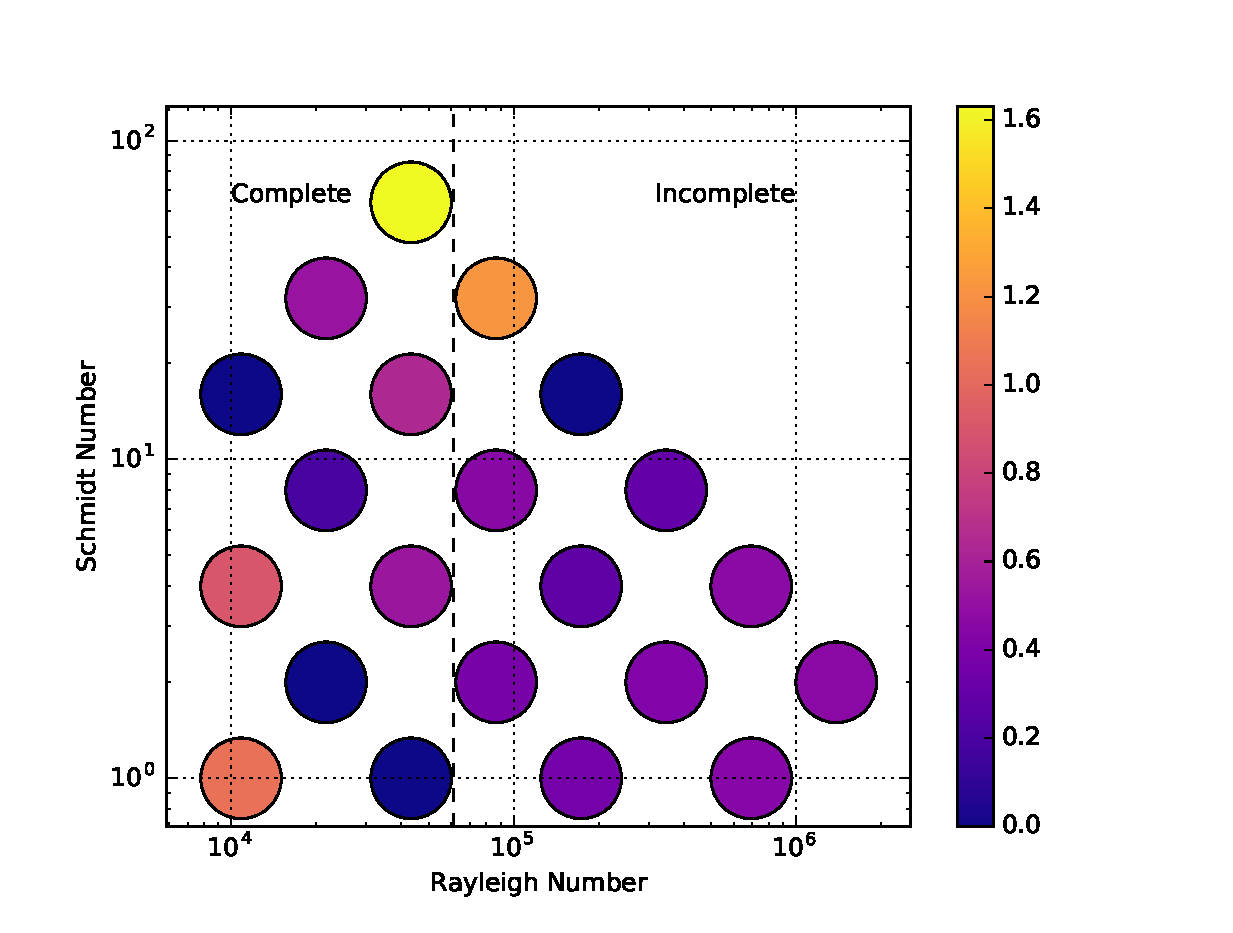
\includegraphics[width=\columnwidth]{figs/C1-vs-Rayleigh-Schmidt}
\caption{ \flabel{C1VsParam}
  Best fit for $C_1$ vs Grashof and Schmidt numbers.
  Experiments on the left side of the dashed line completed when the bubble stopped rising.
  Experiments on the right side of the dashed line are incomplete, having approached the vertical boundaries of the simulated domain.
}
\end{figure}

\begin{comment}
The parameter $C_1$ scales the form drag and serves as a drag coefficient.  
Because we have let $C_0 = 1$, the hydralic diameter of the bubble is roughly $\lambda$.
Had we let $C_0 = 1/4$, the diameter would be the more common $\lambda/2$, but many of the parameters would be fractional.
Now, we relate $C_1$ to the drag coefficient $C_d$ in the drag equation:
\begin{equation}
C_1 \lambda^2 \dot{h}^2 = \frac{1}{2} C_d A \dot{h}^2
\end{equation}
so $C_1$ can be estimated using drag coefficients of cylindrical objects:
\begin{equation}
C_1 = \frac{1}{2} C_d \frac{A}{\lambda^2} = 0.41 \frac{A}{\lambda^2} \approx 0.3
\end{equation}
\end{comment}

The coefficient $C_1$ is related to the drag coefficient $C_d$ as:
\begin{equation}
C_1 = \frac{C_d}{2} \frac{A}{\lambda^2}
\end{equation}

We plot the best fit values of $C_1$ vs the Grashof and Schimdt number in \fref{C1VsParam}.
$C_1$ increases with Grashof and Schmidt number.

\subsubsection{Skin drag coefficient, $C_2$}
\begin{figure}
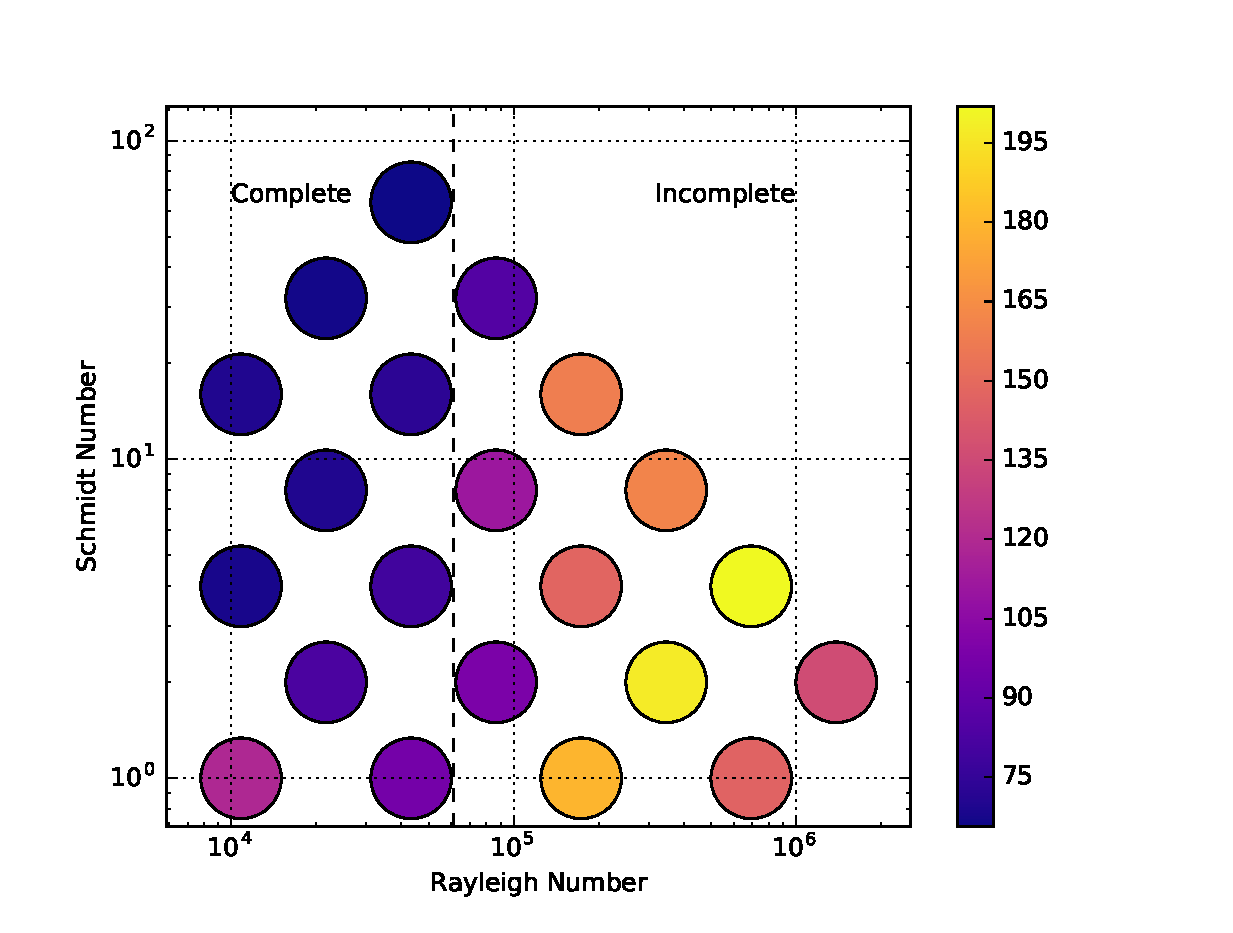
\includegraphics[width=\columnwidth]{figs/C2-vs-Rayleigh-Schmidt}
\caption{ \flabel{C2VsParam}
  Best fit for $C_2$ vs Grashof and Schmidt numbers.
  Experiments on the left side of the dashed line completed when the bubble stopped rising.
  Experiments on the right side of the dashed line are incomplete, having approached the vertical boundaries of the simulated domain.
}
\end{figure}

The coefficient $C_2$ scales the viscous drag, so it is also a drag coefficient of sorts.
$C_2$ sets the terminal velocity in the absence of mixing, so we can relate it to the Darcy friction factor:
\begin{equation}
C_2 = 128 \frac{f_D}{\bar{f}_D},
\end{equation}
where $f_D$ is the Darcy-type friction factor for the bubble and $\bar{f}_D$ is the laminar friction factor for a circular pipe.
If $C_2 < 128$, the rate of momentum transfer out of the bubble is less than circular pipe; for $C_3 > 128$ it is greater.
For the completed trajectories, $C_2$ is about $60$ with only weak dependence on the Rayleigh and Schmidt numbers, while the higher Rayleigh incomplete trajectories have increasing $C_2$.
This suggests that the values of $C_2$ for the incomplete trajectories are underconstrained and will decrease when they are completed.


\subsubsection{Inertial coefficient, $C_3$}
\begin{figure}
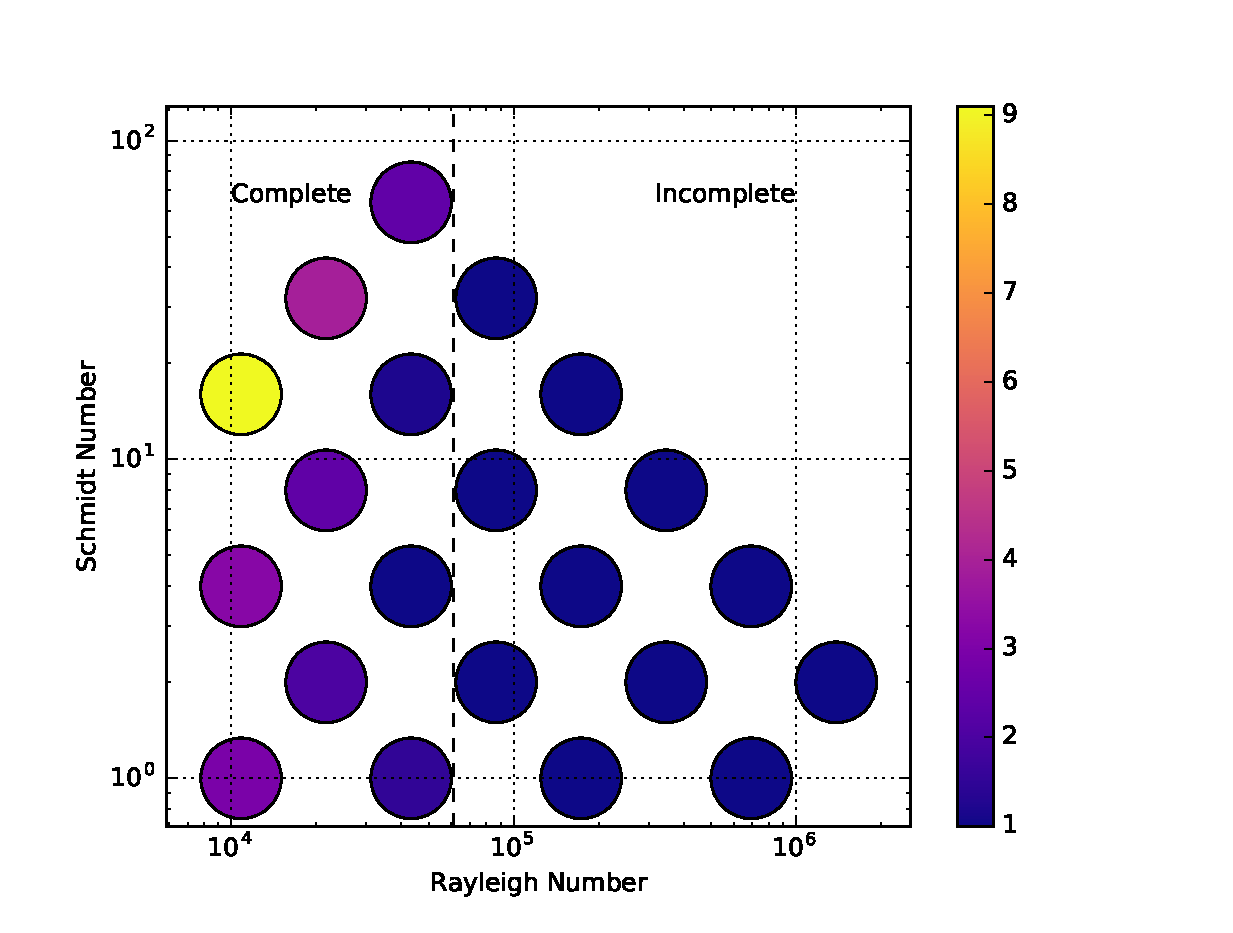
\includegraphics[width=\columnwidth]{figs/C3-vs-Rayleigh-Schmidt}
\caption{ \flabel{C3VsParam}
  Best fit for $C_3$ vs Grashof and Schmidt numbers.
  Experiments on the left side of the dashed line completed when the bubble stopped rising.
  Experiments on the right side of the dashed line are incomplete, having approached the vertical boundaries of the simulated domain.
}
\end{figure}

The coefficient $C_3$ gives the ratio of the inertial height to the buoyant height.
For $C_3 = 1$, the maximum bubble acceleration is $A g$ while $C_3 > 1$ represents the entrainment of neuteraly or anti-buoyant fluid that contributes to the intertia but not the forcing.
Mixing, which also reduces the ratio of the forcing to the inertia, is accounted for explicitly with the $C_5$ coefficient and fit independently to the mixed volume observable, which prevents it from compensating for entrainment.

The majority of trajectories have $C_3 = 1$, indicating that entrainment is not significant.
For completed low Rayleigh high Schmidt flows, however, $C_3$ increases to a value of $2.1$.
The increasing dependence on the Schmidt number and decreasing dependence on the Rayleigh number can be recaste as a decreasing dependence on the Grashof number, independent of the Schmidt number.
This is consistent with the entrainment interpretation of $C_3$, which depends on viscosity but not diffusivity.
We expect the higher Rayleigh trajectories which are incomplete to have increasing $C_3$ at lower Grashof numbers.

\subsubsection{Interfacial area coefficient, $C_5$}
\begin{figure}
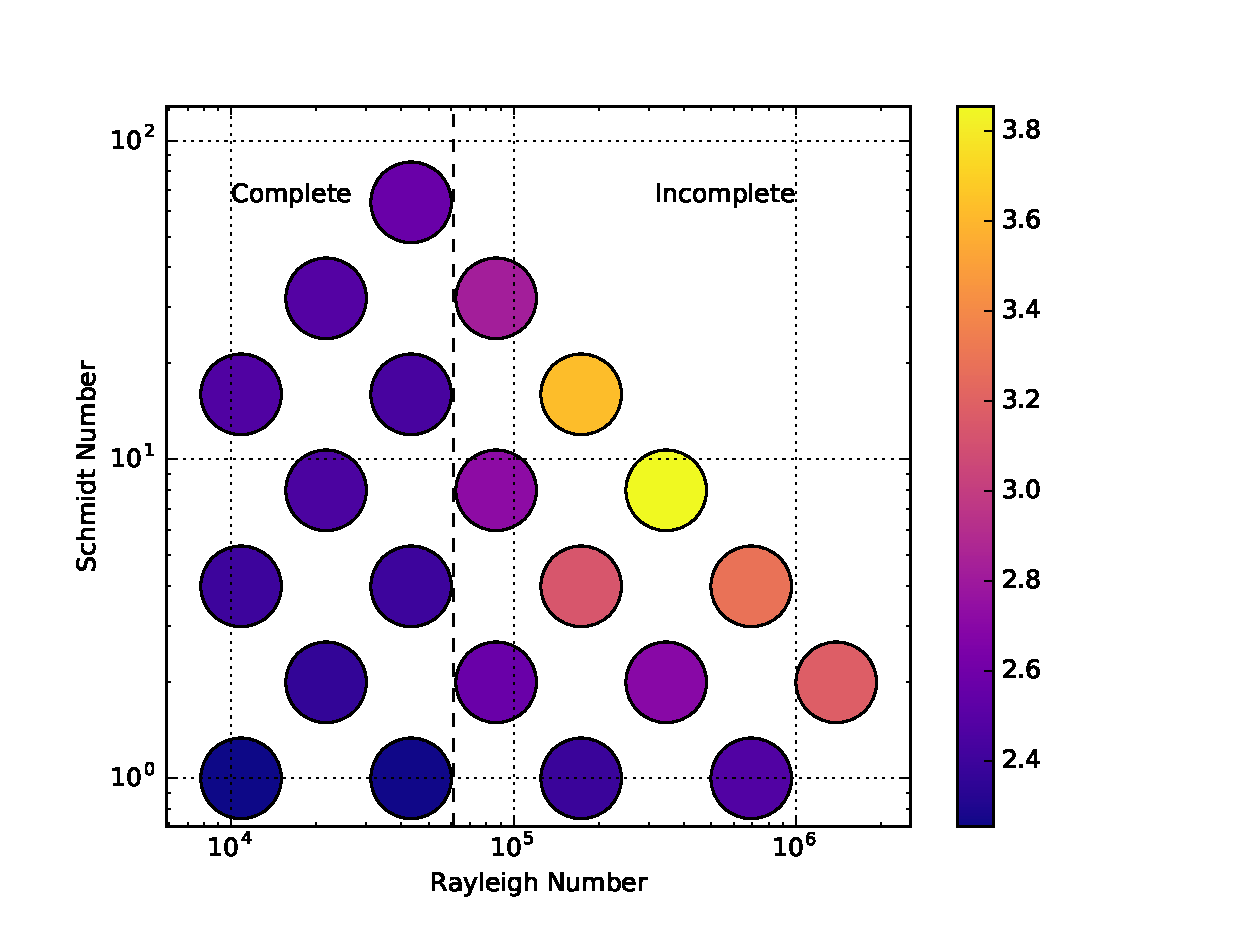
\includegraphics[width=\columnwidth]{figs/C5-vs-Rayleigh-Schmidt}
\caption{ \flabel{C5VsParam}
  Best fit for $C_5$ vs Rayleigh and Schmidt numbers.
  Experiments on the left side of the dashed line completed when the bubble stopped rising.
  Experiments on the right side of the dashed line are incomplete, having approached the vertical boundaries of the simulated domain.
}
\end{figure}

The parameter $C_5$ gives the ratio of the span-wise circumference of the scalar interface to the wavelength.
If the bubble were rectangular in cross section with diameter $\lambda / 2$, then $C_5 = 4$.
Among the completed trajectories, $C_5$ is a much stronger function of the Schmidt number than the Rayleigh number, increasing in both.
The values of $C_5$, which are between 2 and 3, indicate a thinning of the bubble that decreases the mix rate by reducing surface area and total quanity of pure light fluid transported into the dense fluid.

The incomplete trajectories contain richer behavior, with a local maximum at $\text{Ra} = 10^{5.5}$ and $\text{Sc} = 8$.
The the trend of increasing $C_5$ with decreasing diffusivity could imply a wrinkling of the interface that enhances surface area relative to the span-wise are of the bubble.
Similarly, increasing $C_5$ with decreasing viscosity, i.e. increasing Grashof number, could imply that less viscos bubbles have larger span-wise areas, and therefore greater surface area.
The authors have no mechanism by which to explain the local maximum value, so we expect it to disappear with trajectory completition by default.
It would be very interesting if it remained, and further motivates completing the high Rayleigh number trajectories.

\subsubsection{Pure fluid coefficient, $C_7$}
\begin{figure}
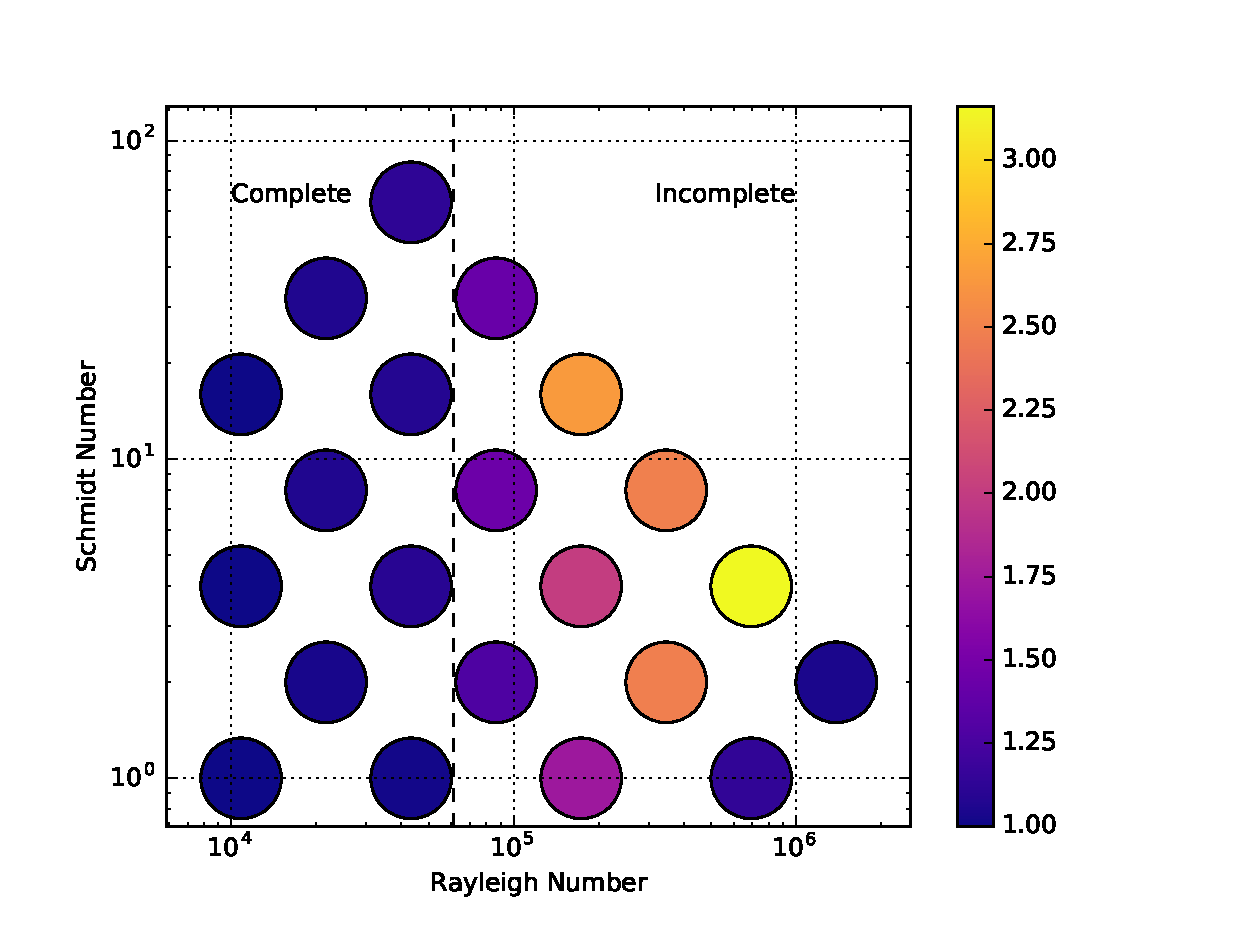
\includegraphics[width=\columnwidth]{figs/C7-vs-Rayleigh-Schmidt}
\caption{ \flabel{C5VsParam}
  Best fit for $C_7$ vs Rayleigh and Schmidt numbers.
  Experiments on the left side of the dashed line completed when the bubble stopped rising.
  Experiments on the right side of the dashed line are incomplete, having approached the vertical boundaries of the simulated domain.
}
\end{figure}

Similar to $C_3$, $C_7$ gives the ratio of the buoyant volume to the maximal mixed volume.
A value of $C_7 = 1$ implies the effective Atwood number is zeroed when $M(t) = \lambda^2 h$.
Values greater than one imply that some portion of the positively buoyant fluid that would be in bubble has become entrained into the neighboring spike, allowing $M(t) > \lambda^2 h$ while retaining net buoyancy.
The complete trajectories all have $C_7 \approx 1$, while the incomplete trajectories at higher Rayleigh numbers have increasing $C_7$.
It is possible that at higher Rayleigh numbers some volume of light fluid detaches from the bubble and is transported into the spike.
However, it is more likely that in the incomplete cases $C_7$, which influences the dynamics most at high mixings, is underconstrained.
In that case, we would expect $C_7 \approx 1$ in all cases. 

